\documentclass[12pt,letterpaper]{article}
\usepackage[spanish,es-nodecimaldot]{babel}
\usepackage[utf8]{inputenc}
\usepackage[T1]{fontenc}
\usepackage{geometry}
\usepackage{graphicx}
\usepackage{amsmath}
\usepackage{booktabs}
\usepackage{float}
\geometry{margin=2.5cm}
\graphicspath{{figuras/}}

\title{Explicación técnica del código de machine learning para el precio del oro}
\author{Alejandro Ramirez \and Leidy Paola Patiño}
\date{\today}

\begin{document}
\maketitle

\section{Objetivo del código}
El archivo \texttt{simulacion\_ml\_mejorada.py} construye un modelo predictivo para el precio del oro. El código toma datos históricos, crea variables explicativas, compara varios algoritmos de machine learning, selecciona el modelo con menor error en validación temporal y genera pronósticos con simulación Monte Carlo.

\section{Carga de datos}
El código lee el archivo \texttt{historicoauplata.xlsx}. Detecta automáticamente la hoja del oro, la columna de fecha y la columna objetivo. También intenta cargar la plata, precios NI 43-101 y variables macroeconómicas de FRED. Las fechas se ordenan cronológicamente para evitar mezclar pasado y futuro.

\section{Variable objetivo}
No se predice directamente el precio del oro. Se predice el log-retorno del precio de cierre al siguiente día hábil:
\begin{equation}
r_{t+1}=\ln\left(\frac{P_{t+1}}{P_t}\right).
\end{equation}
Luego se reconstruye el precio predicho:
\begin{equation}
\hat{P}_{t+1}=P_t e^{\hat{r}_{t+1}}.
\end{equation}
Esto hace que el modelo trabaje con una variable más estable que el nivel del precio.

\section{Construcción de variables}
El código crea rezagos del precio del oro:
\begin{equation}
Lag_k(t)=P_{t-k}.
\end{equation}
También calcula retornos, diferencias, medias móviles y volatilidades:
\begin{align}
R_k(t)&=\frac{P_t}{P_{t-k}}-1,\\
D_k(t)&=P_t-P_{t-k},\\
MA_k(t)&=\frac{1}{k}\sum_{i=0}^{k-1}P_{t-i},\\
\sigma_k(t)&=std(R_1(t-k+1),\ldots,R_1(t)).
\end{align}
Cuando existe plata, se calcula también la relación oro/plata:
\begin{equation}
Ratio_{Au/Ag}(t)=\frac{P_{oro,t}}{P_{plata,t}}.
\end{equation}

\section{Modelos evaluados}
El código compara XGBoost, LightGBM, CatBoost, Random Forest, Extra Trees e HistGradientBoosting. Además, usa Optuna para probar automáticamente combinaciones de hiperparámetros y añadir el mejor candidato encontrado. En el trabajo anterior se seleccionó XGBoost porque presentó el menor error promedio; en esta versión se amplió la comparación y el mejor modelo por validación temporal fue LightGBM optimizado por Optuna.

\section{Validación temporal}
Se usa \texttt{TimeSeriesSplit}. Esto significa que cada fold entrena con observaciones antiguas y valida con observaciones posteriores. No se usa partición aleatoria porque en series de tiempo eso produciría fuga de información.

\section{Métricas}
El código calcula MAE, RMSE, MAPE y $R^2$:
\begin{align}
MAE &= \frac{1}{n}\sum |y_i-\hat{y}_i|,\\
RMSE &= \sqrt{\frac{1}{n}\sum (y_i-\hat{y}_i)^2},\\
MAPE &= \frac{100}{n}\sum \left|\frac{y_i-\hat{y}_i}{y_i}\right|.
\end{align}

\section{Pronóstico recursivo}
Para pronosticar a futuro, el modelo parte del último precio observado. Predice el retorno del siguiente día, reconstruye el precio y agrega ese precio a la serie. Después repite el proceso:
\begin{equation}
P_{t+1}=P_t e^{\hat{r}_{t+1}}.
\end{equation}
Este procedimiento permite extender la trayectoria hasta 2035.

\section{Monte Carlo}
La simulación Monte Carlo agrega incertidumbre al retorno base:
\begin{equation}
r_t^{MC}=\hat{r}_t+\epsilon_t\sigma_s+J_t.
\end{equation}
Aquí $\epsilon_t$ es un choque aleatorio, $\sigma_s$ es la volatilidad del escenario y $J_t$ es un salto aleatorio ocasional. Después se calcula el precio simulado:
\begin{equation}
P_t^{MC}=P_{t-1}^{MC}e^{r_t^{MC}}.
\end{equation}

\section{Archivos generados}
El código genera archivos CSV, Excel, gráficas PNG y el modelo entrenado en formato \texttt{joblib}. Las salidas principales quedan en \texttt{resultados/} y las gráficas en \texttt{resultados/graficas/}.

\begin{figure}[H]
\centering
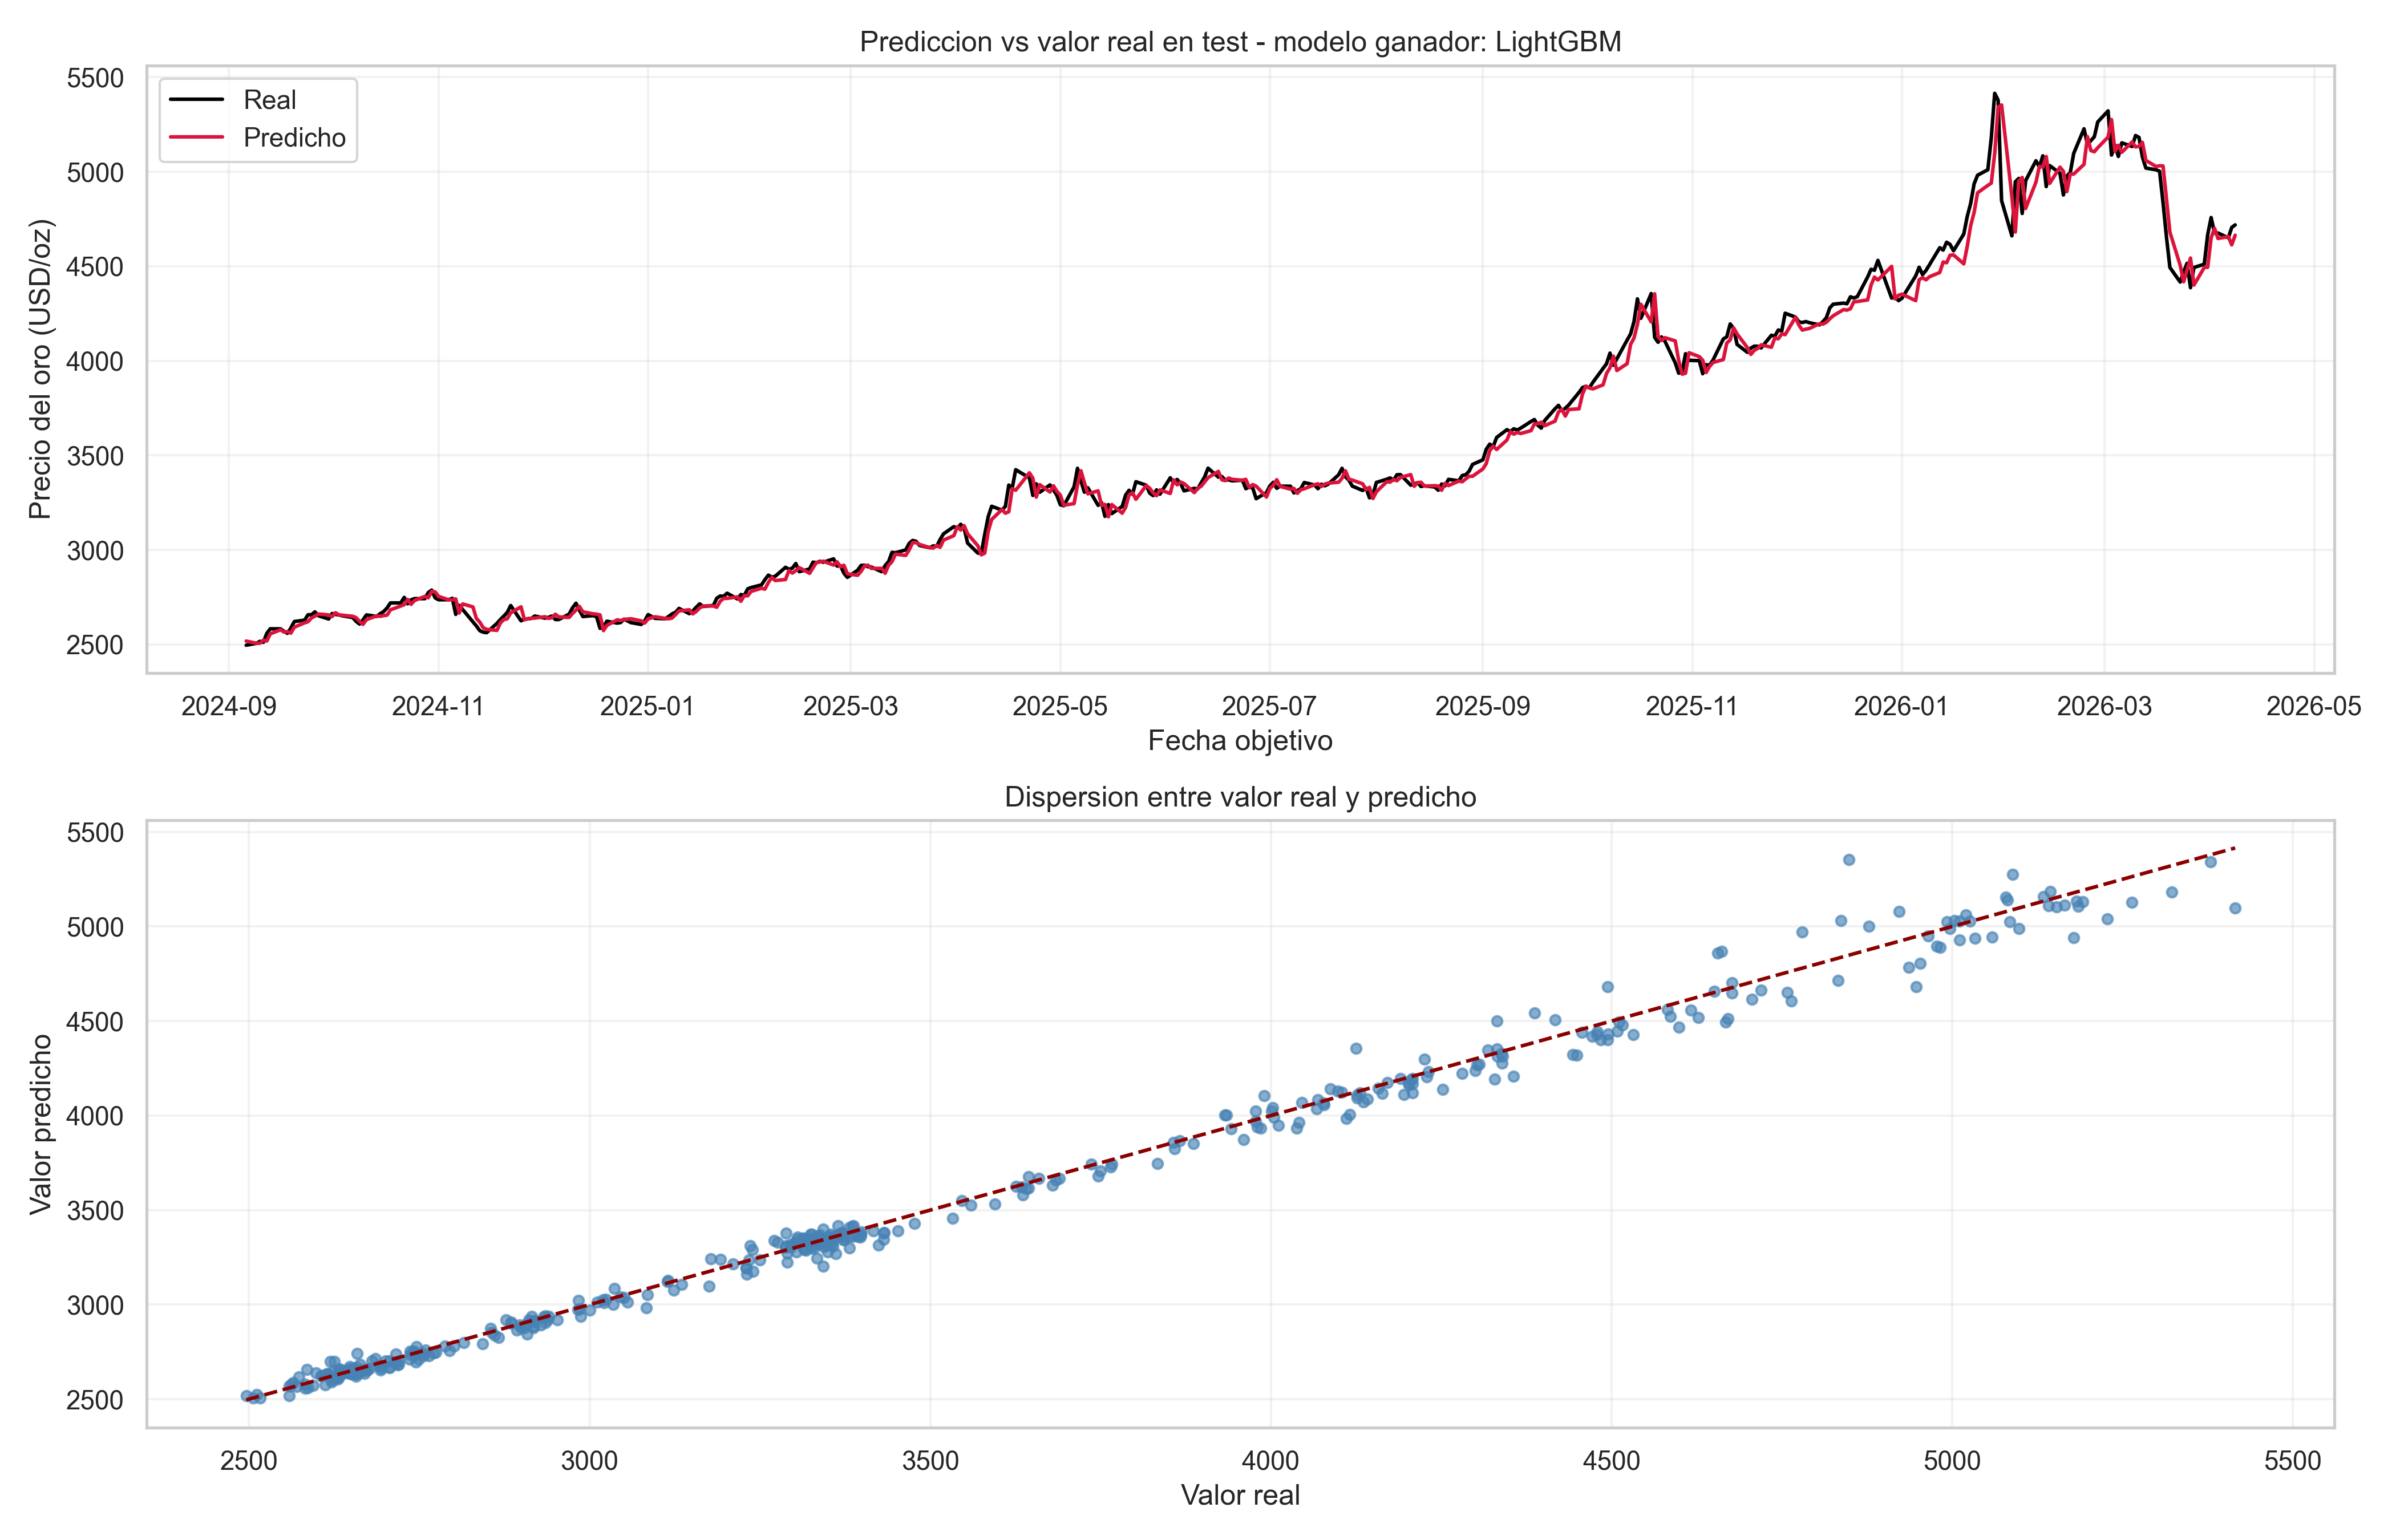
\includegraphics[width=0.95\textwidth]{02_prediccion_vs_real_test.png}
\caption{Validación visual del modelo en la ventana de prueba.}
\end{figure}

\begin{figure}[H]
\centering
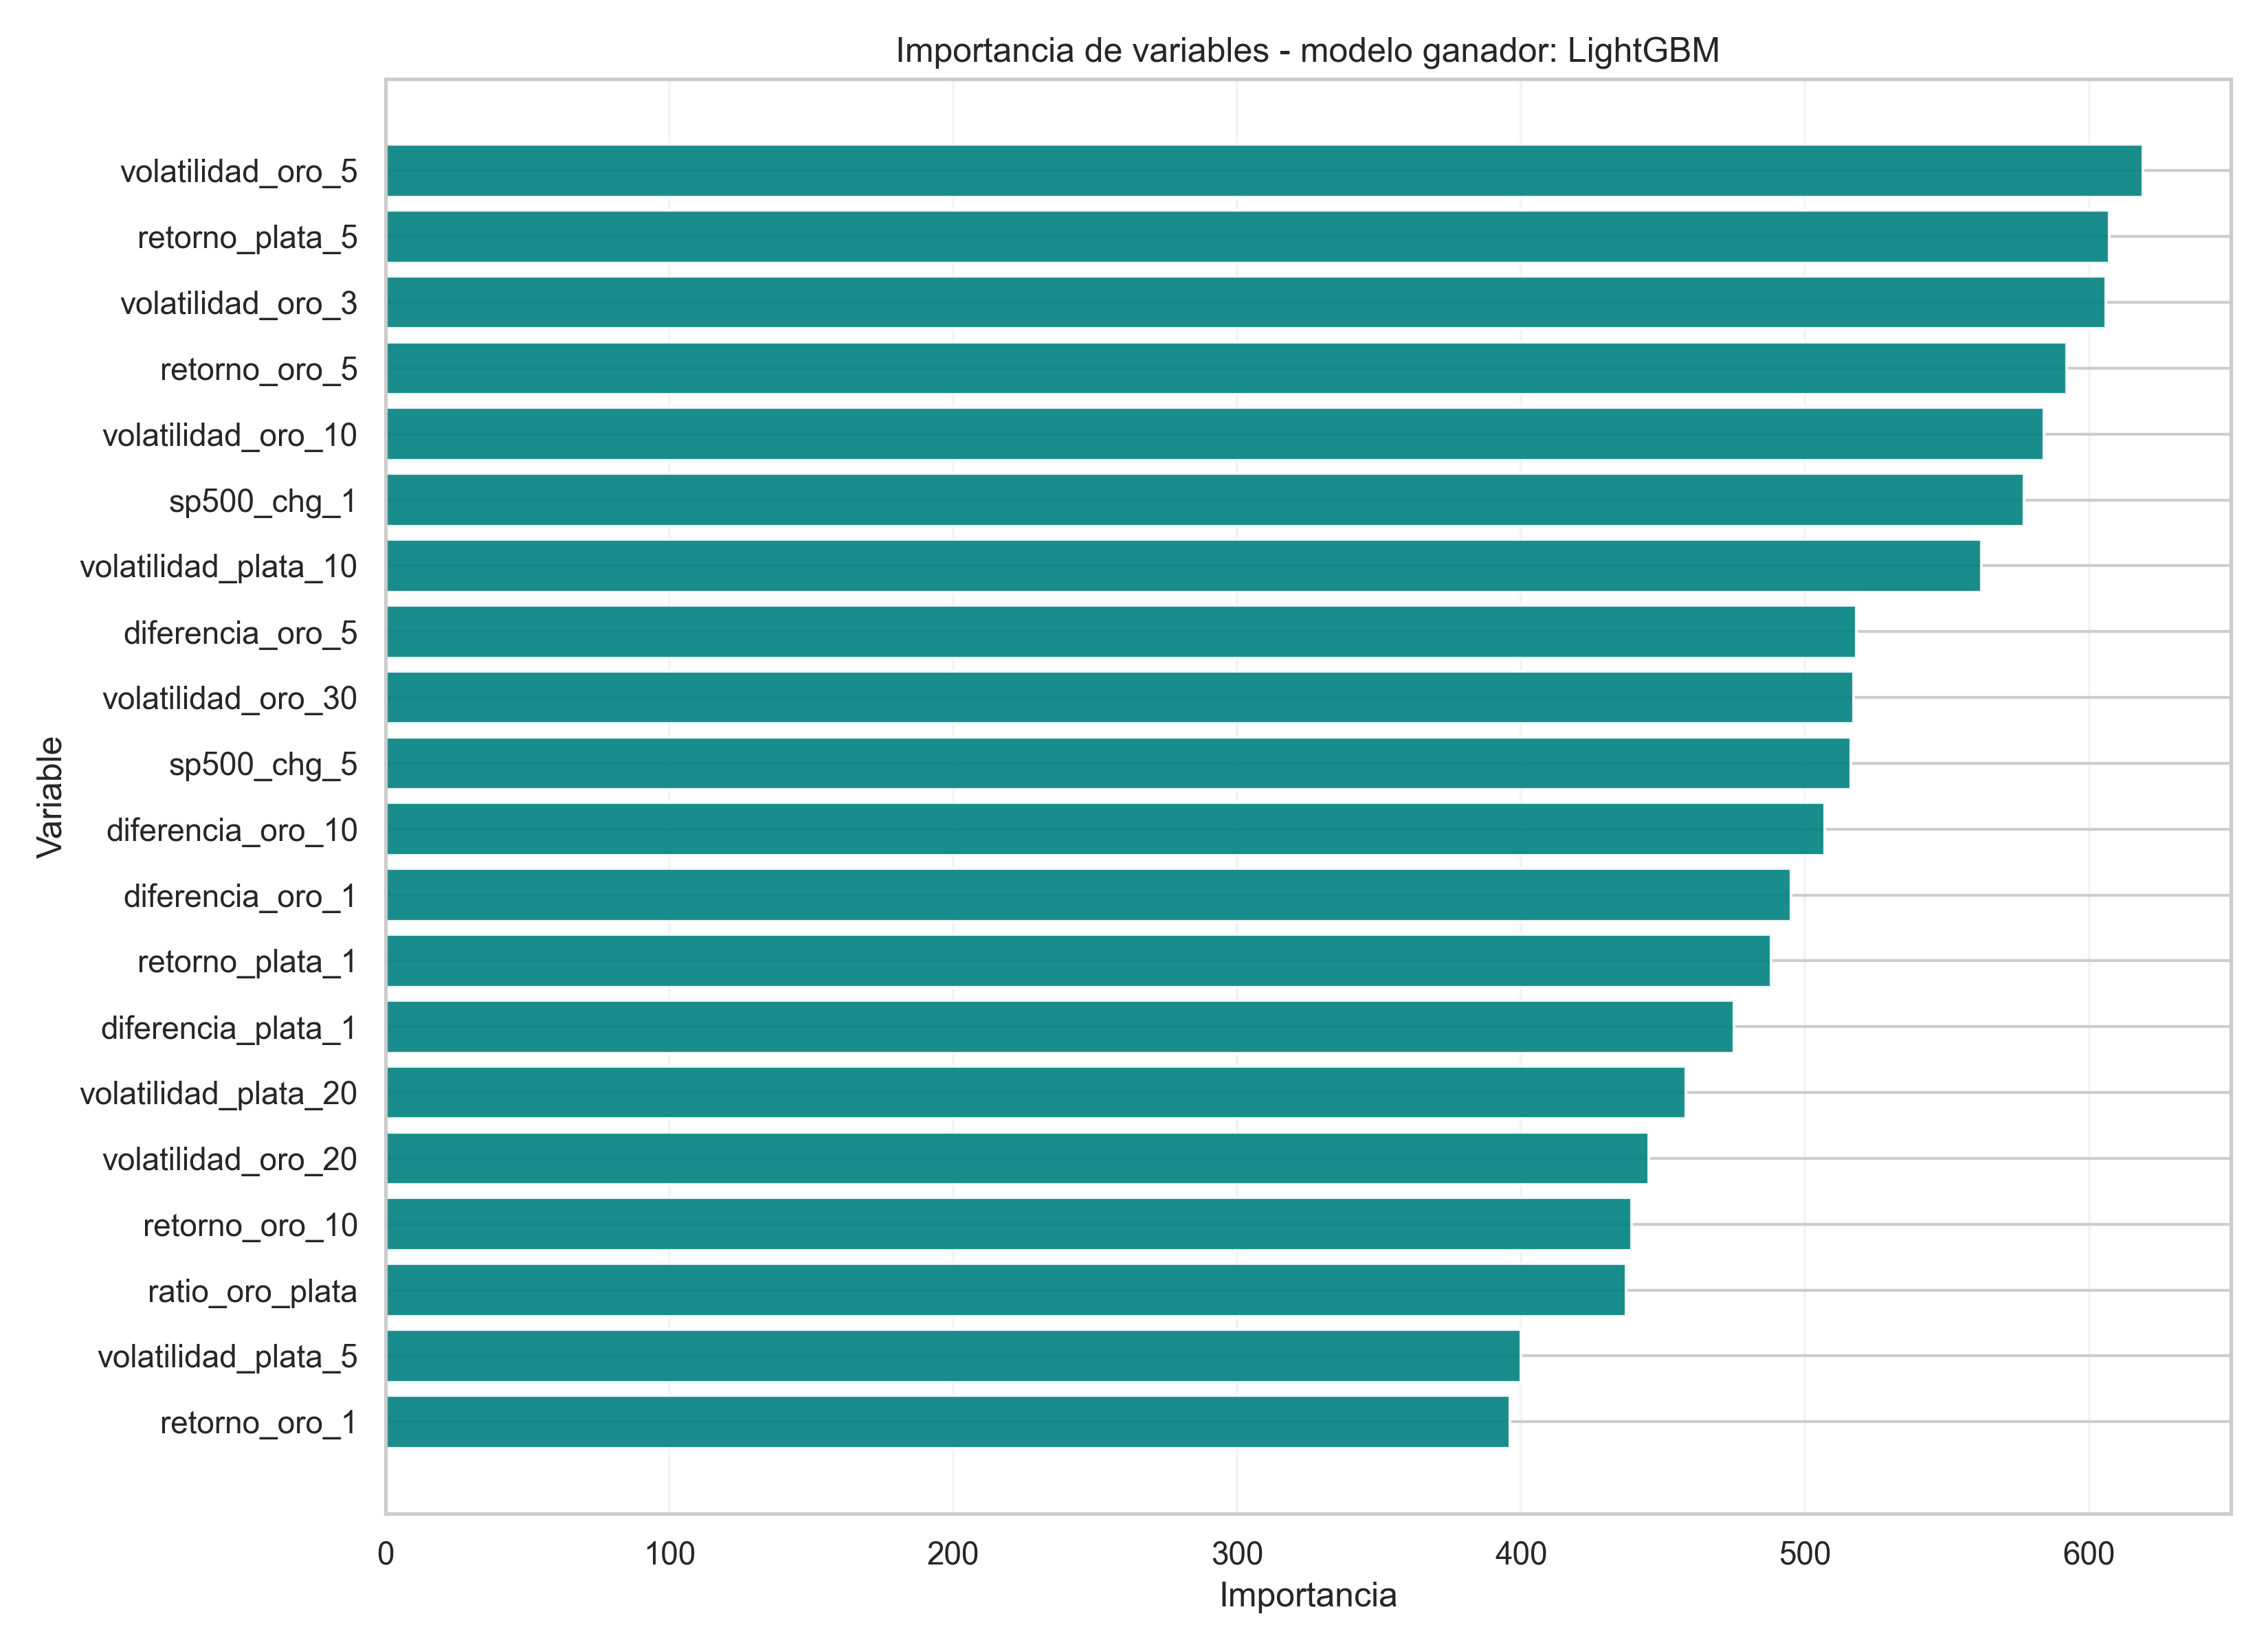
\includegraphics[width=0.95\textwidth]{04_importancia_variables.png}
\caption{Variables más importantes usadas por el modelo seleccionado.}
\end{figure}

\end{document}
